\section{Analysis} 
In this section, we present the system under consideration, describe our analysis method, and discuss the results of our work.


\subsection{Injection signal}
\label{Injection_signal}

The system we consider in this work is a MBHB characterized by the following physical quantities:

\begin{itemize}
\item total mass $M$ and mass ratio $ q$ of $2 \times 10^6 M_\odot $ and 2, respectively,
\item BHs spins $\chi_1 = \chi_2 = 0.3$,
\item inclination angle $\iota = \pi/3$ and azimuthal direction $\phi_0 = 0$,
\item longitude $\lambda$, latitude $\beta$, and polarisation $\psi$ all equal to $\pi/3$;

\end{itemize}

the luminosity distance, $D_L$,  is set such that the full signal has an SNR of 600.
The total mass has been chosen to have a GW signal that accumulates a significant SNR amount in the inspiral portion, unlike more massive binaries where the most significant SNR contribution comes from the merger part of the signal. We stress that this system does not represent a realistic astrophysical choice since the long-wavelength approximation for the LISA response is expected to break for $ M \sim 10^6 M_\odot$. Despite this, for the purpose of our analysis into seeking and removing false GR deviations, the approximation break is not an obstacle, since we refers to a property of the system itself, not to the interaction between the signal and the detector. We choose an SNR of 600 to observe a relative high value for the false GR deviations.

The GW signal produced by this source will be the injection signal for the analysis. We restrict only to the (2, 2) harmonic, since it is the dominant one. A visual representation is given in Fig. \ref{fig:Injection_division}. There, we can see the increase of the GW amplitude while approaching the BHs plunge alongside with the signal frequency increase. The strong damping of the signal immediately after the merger is also evident.

\begin{figure}[h!]
    \centering
    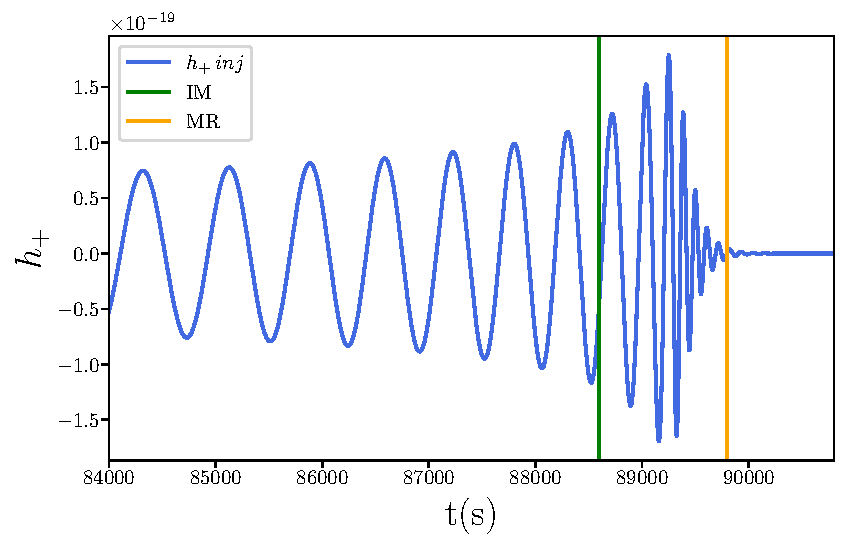
\includegraphics[width=0.7\textwidth]{Images/Injection_division.pdf}
    \caption{Real component of the strain, $h_+$, versus the time of the signal. The visualization is restricted around the merger time. Vertical lines are the divisor between different parts of the signal, IM = inspiral-merger; MR= merger-ringdown.}
    \label{fig:Injection_division}
\end{figure}


\subsection{Parameter estimation on the full signal}

We perform Bayesian parameter estimation using MCMC to infer the posterior distributions of the pSEOBNRv5HM model parameters. We make use of the \texttt{Eryn} sampler, as introduced in sec. \ref{Bayesian_Analysis}. Regarding the sampling mechanism, it consists of two initial burn-in phases of 500 iterations, followed by an effective sampling run of 6000 iterations.
The burn-in phases are used to allow the Markov chains to converge toward the target posterior distribution.

The sampling is carried out simultaneously by 42 walkers. Their initial positions in parameter space are drawn from a Gaussian distribution centred on the true values for all parameters being recovered, except for the fractional deviation parameters, which are initialized from their respective uniform priors. If, after 20 tries the Gaussian drawn parameters are not in the respectively prior range, they are drawn from their uniform priors.

In Fig. \ref{fig:Corner_inj_snr_600_M_2e6}, we show the corner plot for the system described in sec. \ref{Injection_signal}, illustrating the joint 2D distributions and, on the diagonal, the marginalised distribution for each one of the recovered model parameters. Among the eleven parameters, many are accurately recovered. The comparison is done looking at the green and orange lines, meaning the truth injection values and the maximum $ \log \mathcal{L}$ set of parameters, respectively. Other ones are biased, such as the total mass $M$. Mainly we can observe the false detection of GR fractional deviations. A summary statistic for these deviations is given by

\begin{equation}
\delta f_{22} = -0.030^{+0.009}_{-0.009} \,, \quad 
\delta \tau_{22} = -0.029^{+0.019}_{-0.021} \,;
\end{equation}

\noindent 

where we report the $0.05$, $0.5$, and $0.95$ quantiles of the posterior distribution, defining a $90\%$ credible interval.

\begin{figure}[h!]
    \centering
    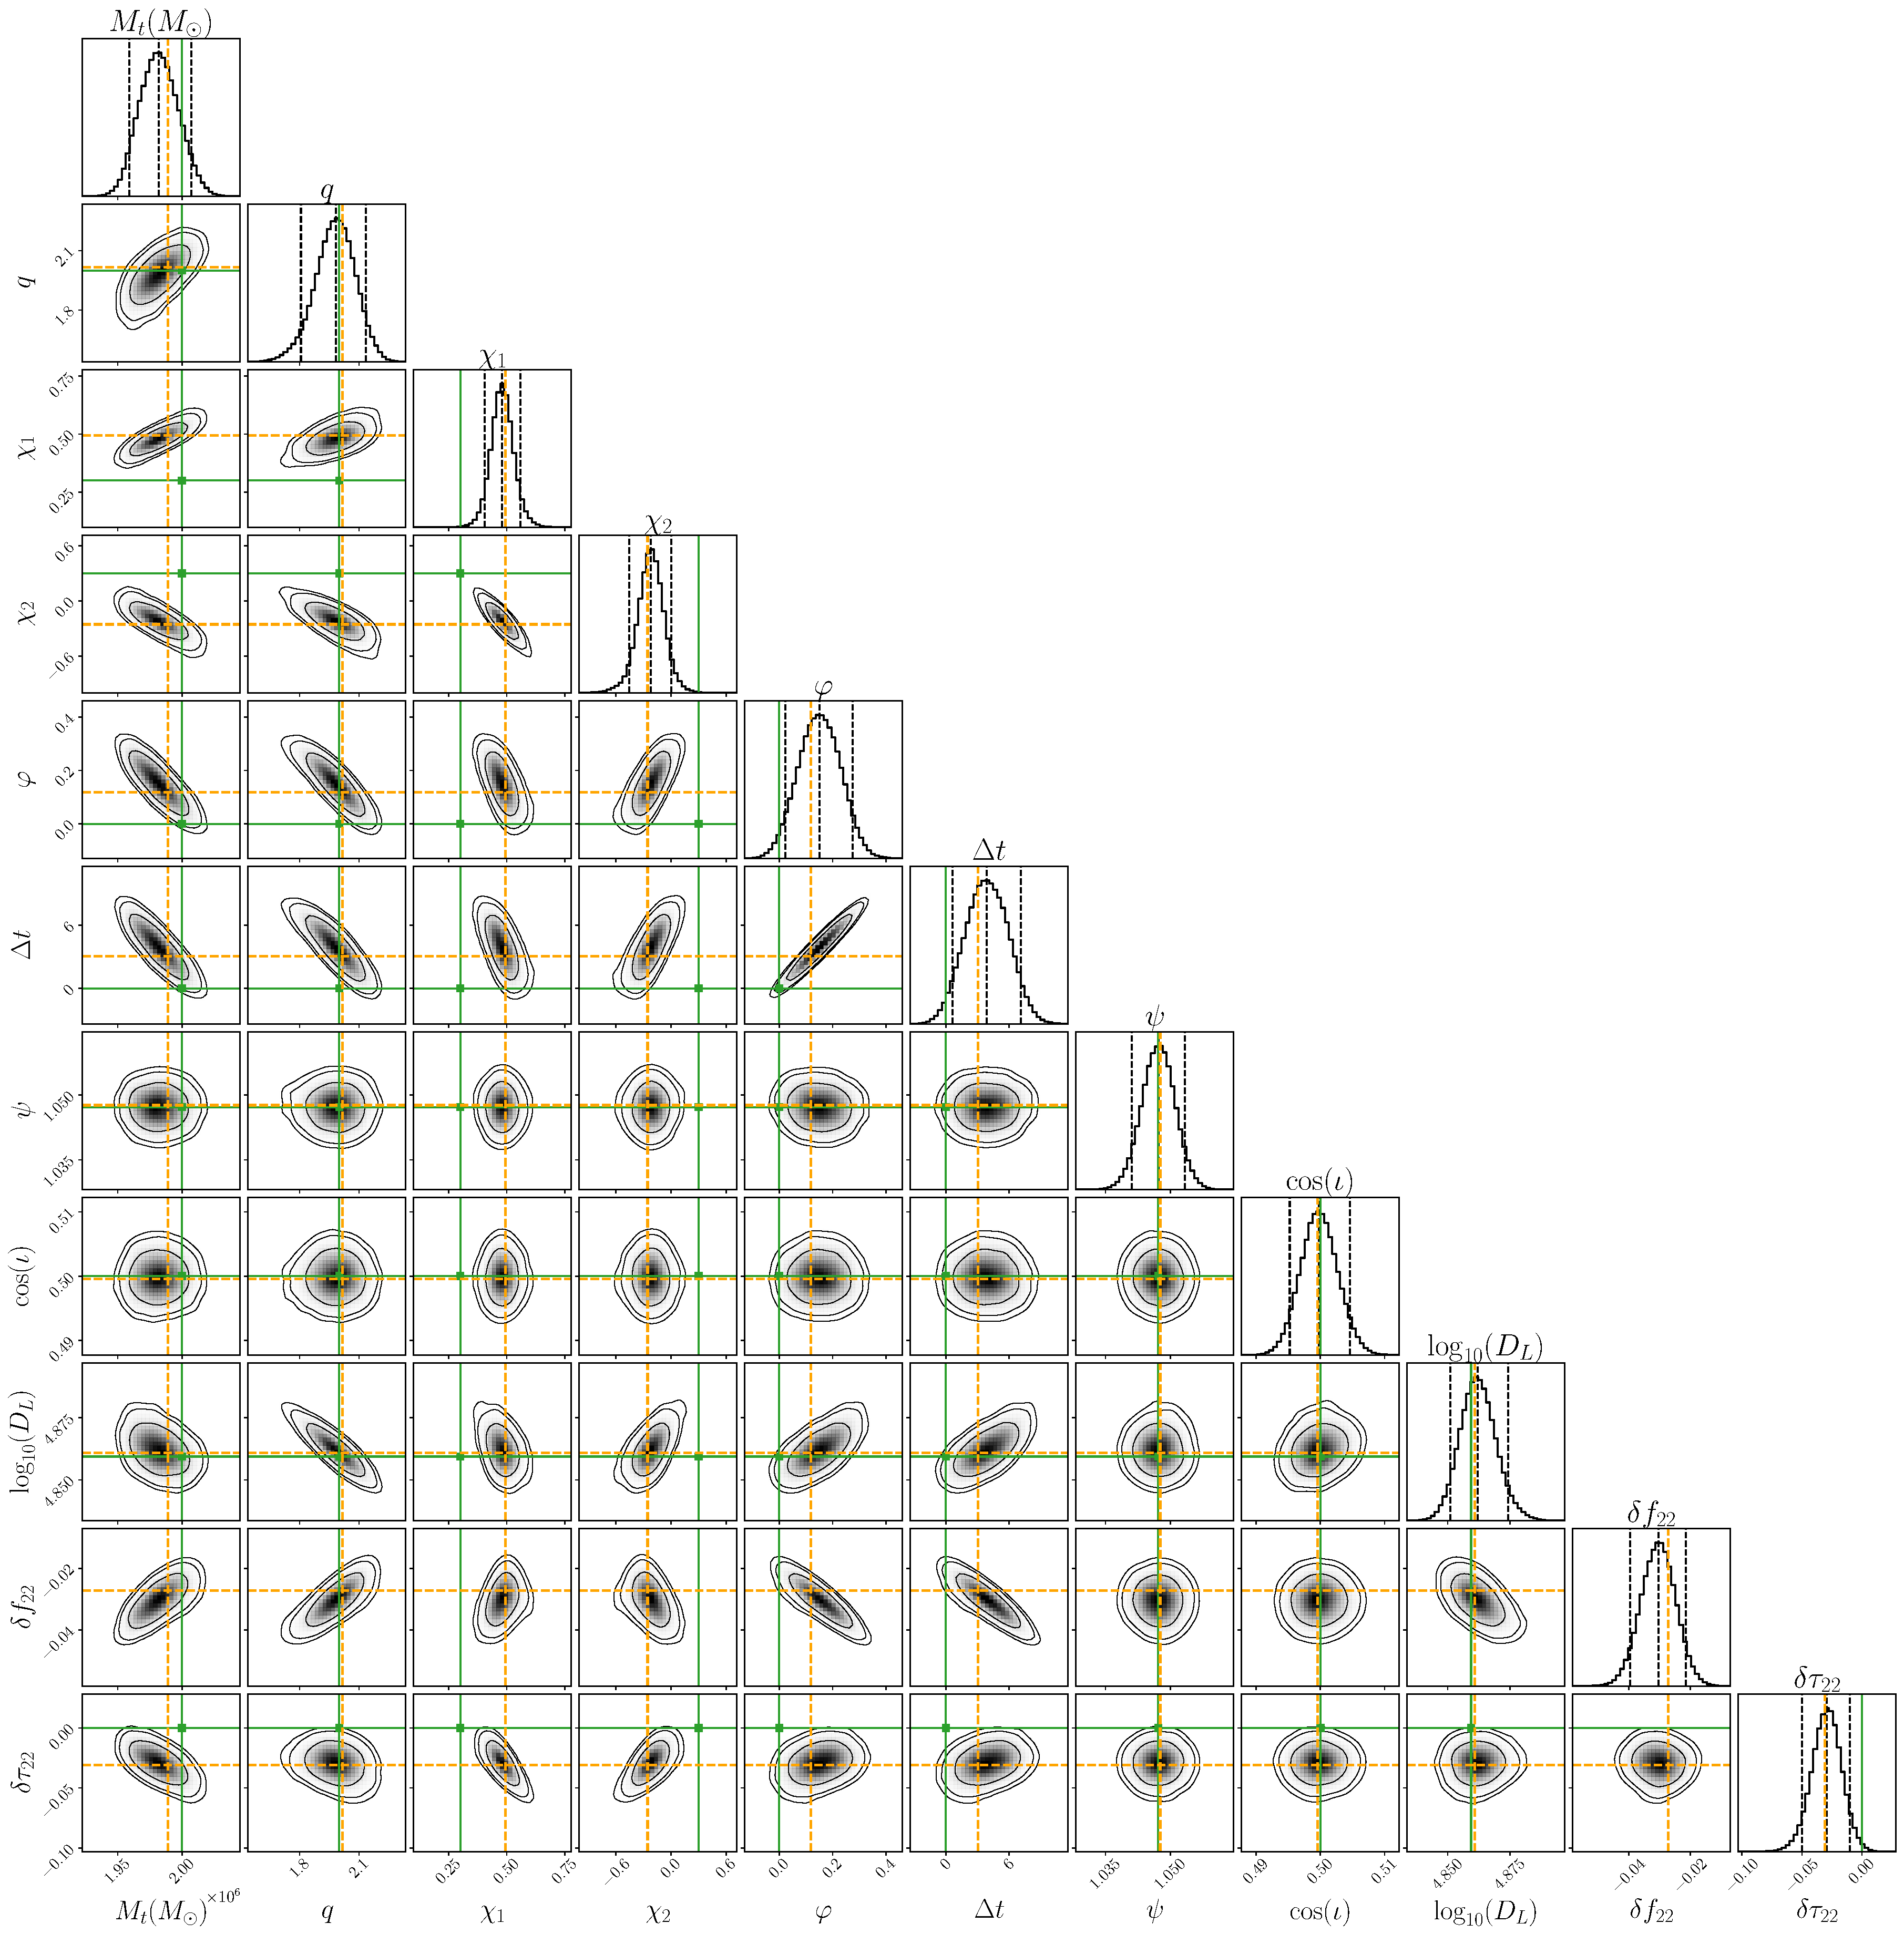
\includegraphics[width=1\textwidth]{Images/Corner_inj_snr_600_M_2e6.pdf}
    \caption{Corner plot for the injection system. Contours show the $68\%$, $90\%$, and $95\%$ confidence intervals. The black dashed lines represent the $0.05$, $0.5$, and $0.95$ quantiles. The green lines show the injection true parameters, the orange ones the maximum $ \log \mathcal{L}$ set of parameters.}
    \label{fig:Corner_inj_snr_600_M_2e6}
\end{figure}



\subsection{Frequency cut investigation}


We observed that considering the full injection signal produces a biased result. It is also worth noting that that our sampling method is performed by maximizing the $\log \mathcal{L}$ function, which describes how much the injection and the recovered signal, i.e. a EOB waveform built according to the sampled set of parameters, are similar. The $\log \mathcal{L}$ is proportional to the square of the SNR of a given portion of the signal, this leads to the sampler to prefer matching the merger part of the signal rather than the inspiral part, since it is the loudest part of the signal. By construction, the EOB formalism should give a good description of the inspiral portion of the signal. Following this reasoning, we will proceed with the analysis by performing a sampling run not on the full signal, but instead only in the inspiral. 

In order to do such cut on the signal, we need to identify a division between the inspiral and the merger, so the  corresponding frequency since the $\log \mathcal{L}$ is done in frequency domain. Looking at Fig. \ref{Injection_signal}, we can observe two vertical lines. The green one represents the division between the inspiral portion to the merger one, instead the yellow line divides the merger to the ringdown part. These divisions are done in time domain and they are arbitrary, the lack of an unambiguous separation is irrelevant for our purposes.

We can start from the following expression:

\begin{equation}
\phi = \tan^{-1} \left( \frac{ h_{\times}}{ h_{+}} \right) \,, \quad
f_{\text{gw}}(t) = \frac{1}{2\pi} \frac{d\phi(t)}{dt} \,;
\end{equation}

\noindent
to obtain the signal frequency as a function of time. In Fig. \ref{fig:Frequency_cut}, we can observe two different frequency trends. The oscillatory behaviour of the blue line is due to the harmonics considered in the signal. When we consider only the (2,2) harmonic, we implicitly assume the counter-rotating harmonic (2,-2). The orange line does not present this behaviour because we imposed the inclination $\iota$ to be 0, only seeing the (2,2) mode.
The red horizontal line is our value of the cut frequency, $f_{cut} = 0.00025$. This variable will be the final value at which the likelihood will be computed in our bayesian analysis.

\begin{figure}[h!]
    \centering
    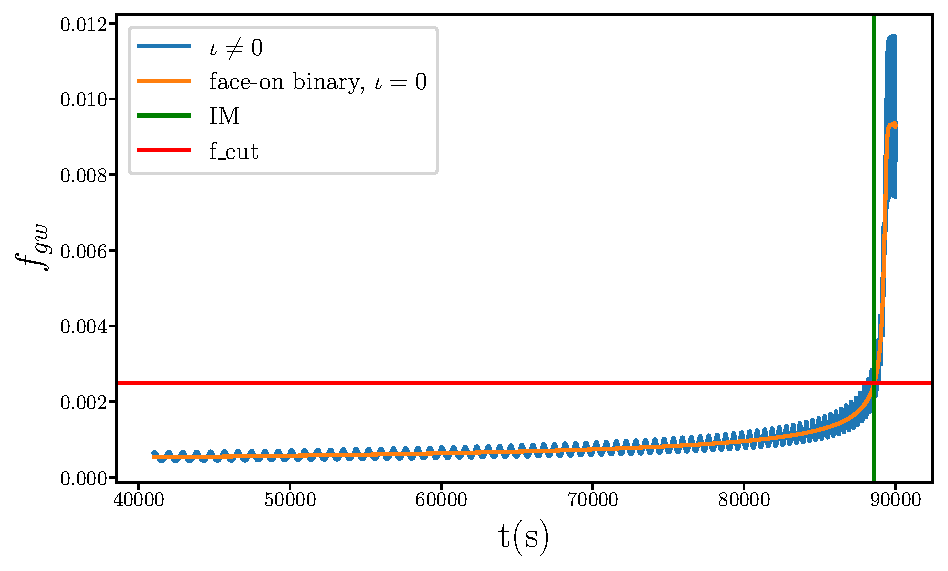
\includegraphics[width=0.7\textwidth]{Images/Frequency_cut.pdf}
    \caption{Plot of the frequency versus time. The blue line is for the signal with (2,2) and (2,-2) harmonics, the orange one is for the same signal but with $ \iota = 0$. The red horizontal line is the $f_{cut}$ value. }
    \label{fig:Frequency_cut}
\end{figure}



\subsection{Parameter estimation on the inspiral portion}

After determining the frequency value at which to stop the $\log \mathcal{L}$ computation, we perform a second, analogous Bayesian parameter estimation run, using the same sampler. The injection signal has the same characteristic as before, with the exception of rescaling the luminosity distance of the source, in order to impose an SNR of 600 for the signal until $f_{cut}$. To determine the appropriate rescaling for this value, we proceed as follows: we compute the SNR for the all injection signal where we imposed an SNR of 600 until $f_{cut}$, and use it to rescale the injection such that the SNR becomes 600 for the full signal. The same rescale factor is then used to correctly adjust the luminosity distance.
The rescaling is motivated by the need to maintain consistency in the $\log \mathcal{L}$ comparison between the different runs. We present the corner plot of this run in Fig. \ref{fig:Corner_full_fcut}. We can immediately observe that the ranges of the posteriors are broader, when compared to the run on the full signal. One possible reason for this observation is that we lack a portion of the signal, i.e. the merger part, that is very informative about the parameters. There is also a huge difference in the $\log_{10} D_L$ posterior, due to the rescaling procedure previously discussed. Lastly, the $\delta \tau_{22}$ marginalised posterior remains flat as the prior, suggesting this parameter is not actually involved in the $\log \mathcal{L}$ computation, as we expected by truncating before QNM gets involved. 



\begin{figure}[h!]
    \centering
    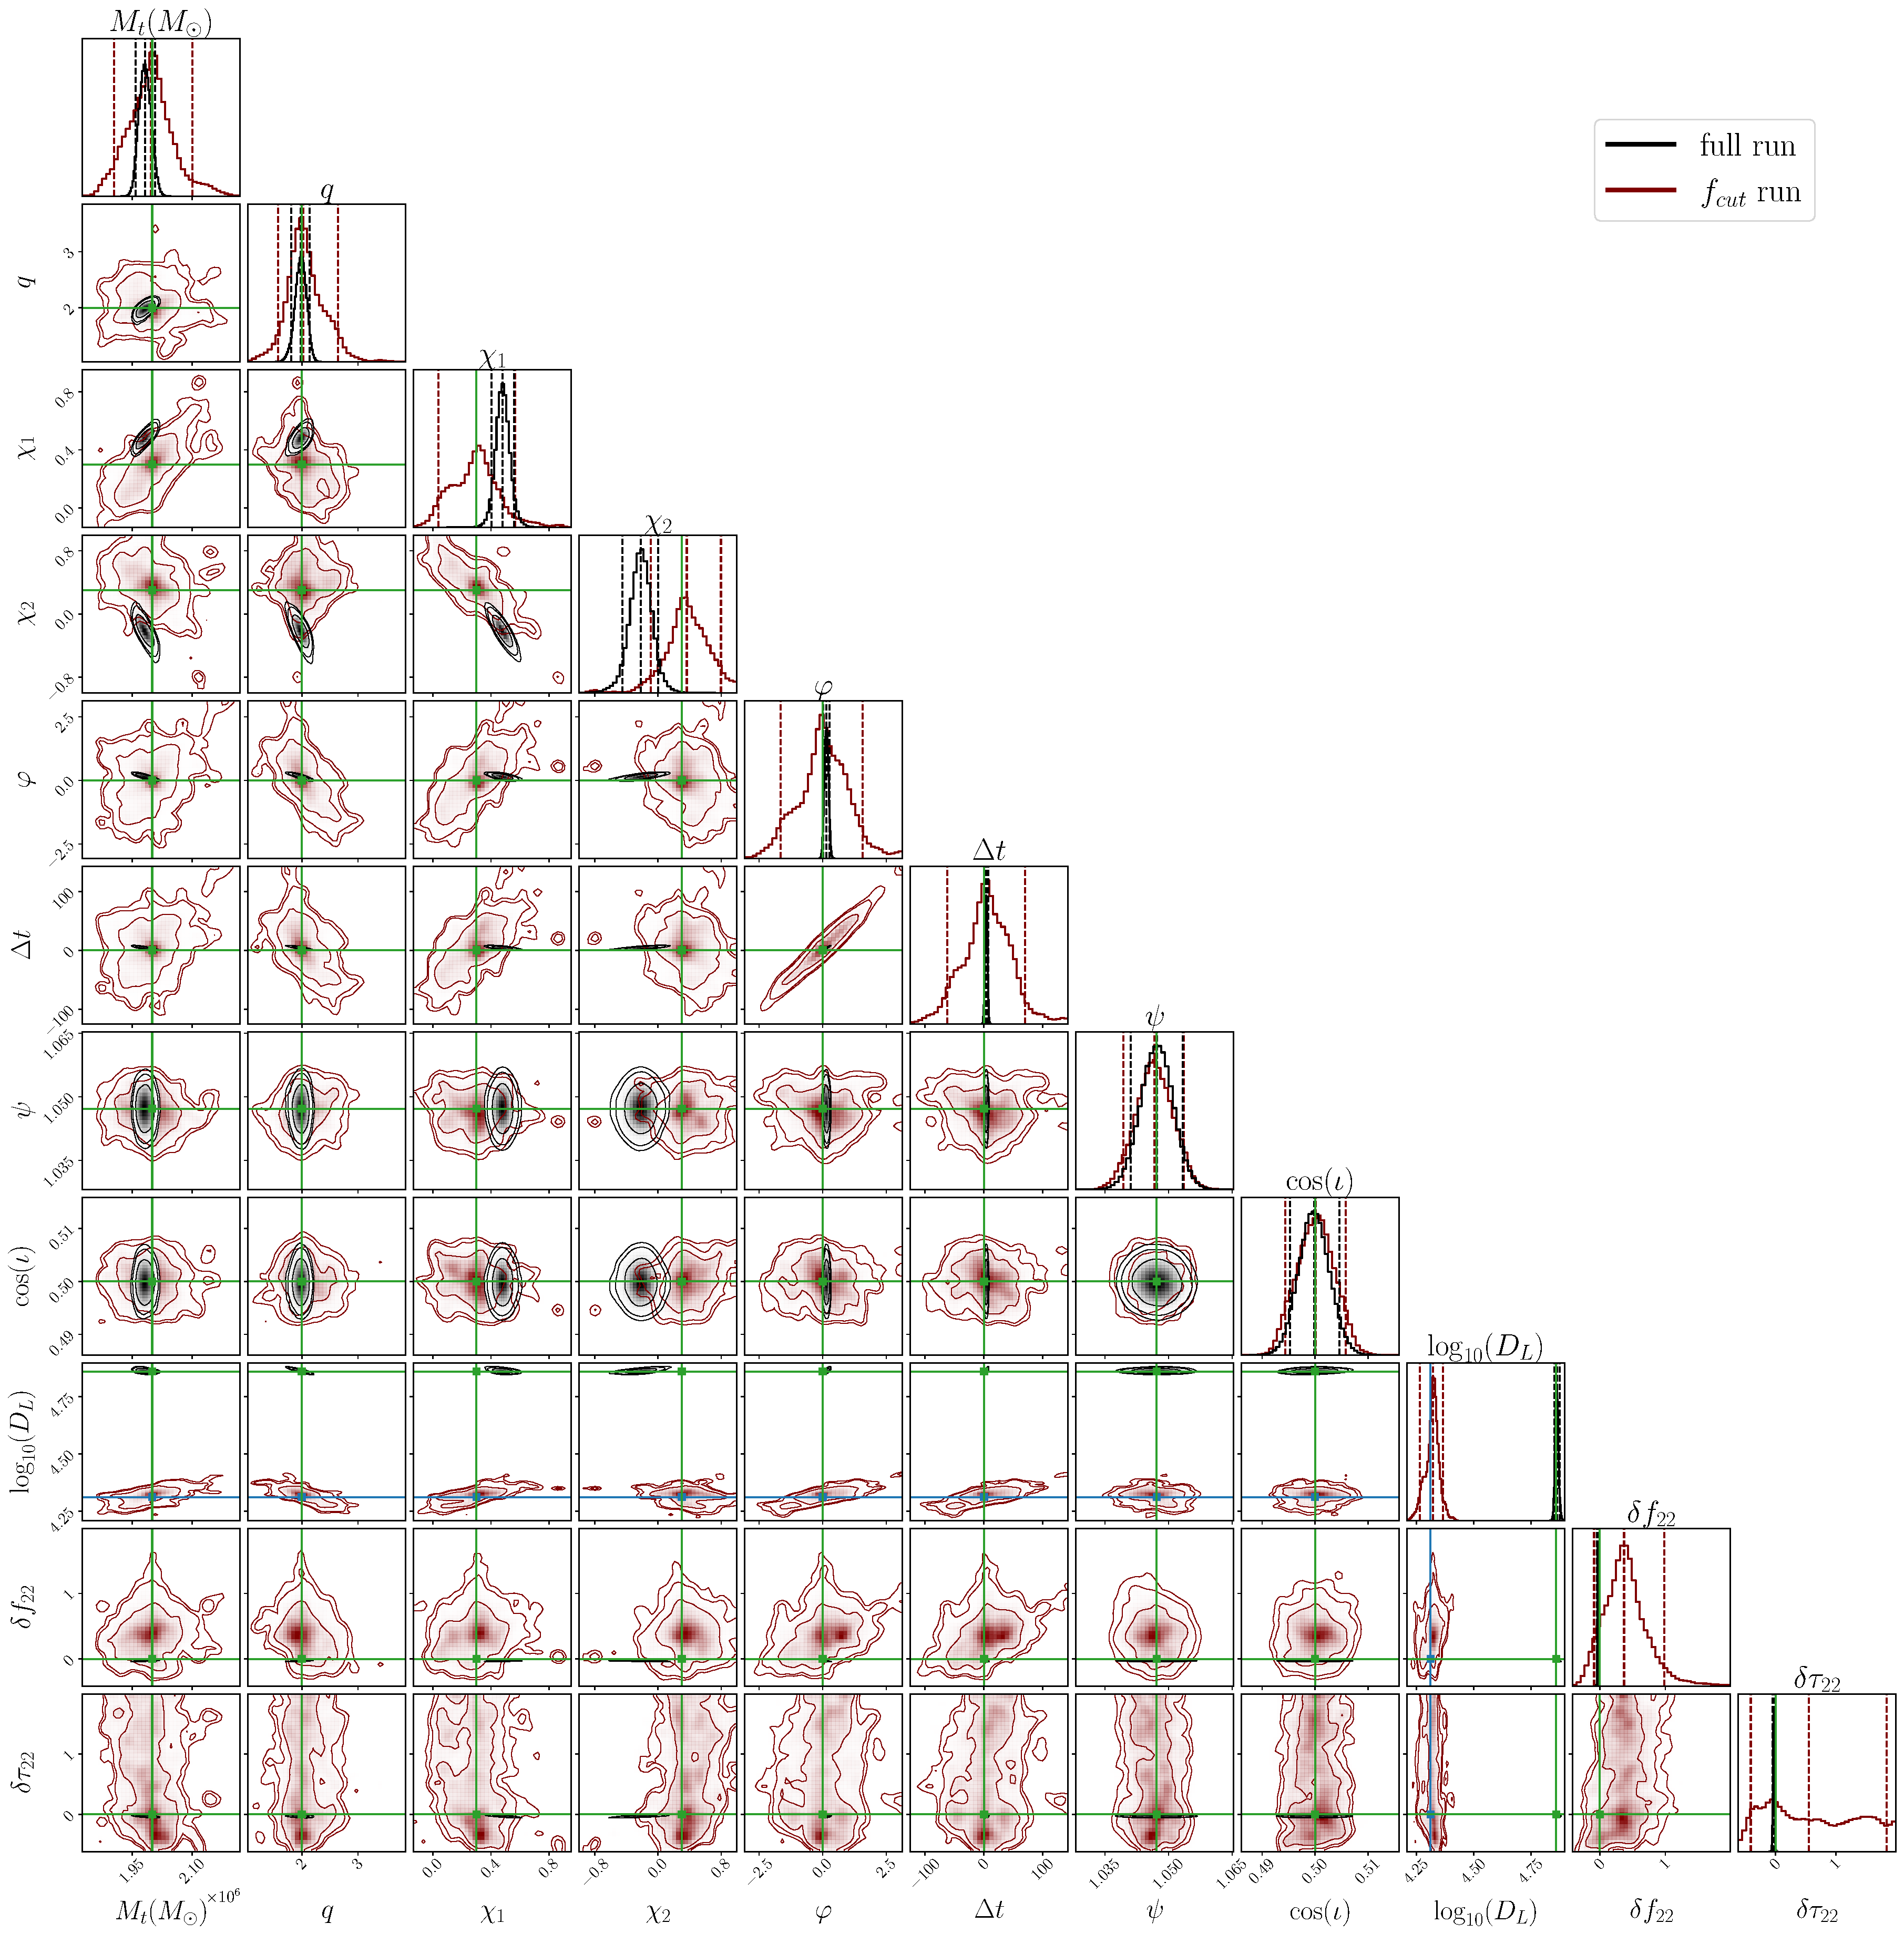
\includegraphics[width=1\textwidth]{Images/Corner_full_fcut.pdf}
    \caption{Corner plots for the injection system. Black/red colors represent the full run and the run until $f_{cut}$ . Contours show the $68\%$, $90\%$, and $95\%$ confidence intervals. The black/red dashed lines represent the $0.05$, $0.5$, and $0.95$ quantiles. The green lines show the injection true parameters.}
    \label{fig:Corner_full_fcut} 
\end{figure}


From this run, we take the maximum $\log \mathcal{L}$ set of parameters and we will use them to generate a waveform to carry on our analysis. From this set, the $\log_{10} D_L$ value needs to be modified if we want to compare this waveform to the original injection, following the same procedure described above.  

When we create this waveform we also impose the fractional deviation parameters to be $0$, since the parameter estimation run is done in a signal portion where they are irrelevant.

Looking at Fig. \ref{fig:Inj_best_insp}, we have a visual comparison between the injection signal and the waveform generated by the best set of inspiral parameters, which we will refer to as the best inspiral waveform. This comparison is presented in form of $h_{+}$ and $h_{\times}$. From a quantitative point of view, the agreement of this waveform to the inspiral part of the injection is described by a $\log \mathcal{L}$ value of $ -0.55$. In contrast, for the full signal we find $\log \mathcal{L} = -2377.59$, suggesting an inaccurate description of the merger that can be improved by the fractional deviations and wavelets.

\begin{figure}[h!]
    \centering
    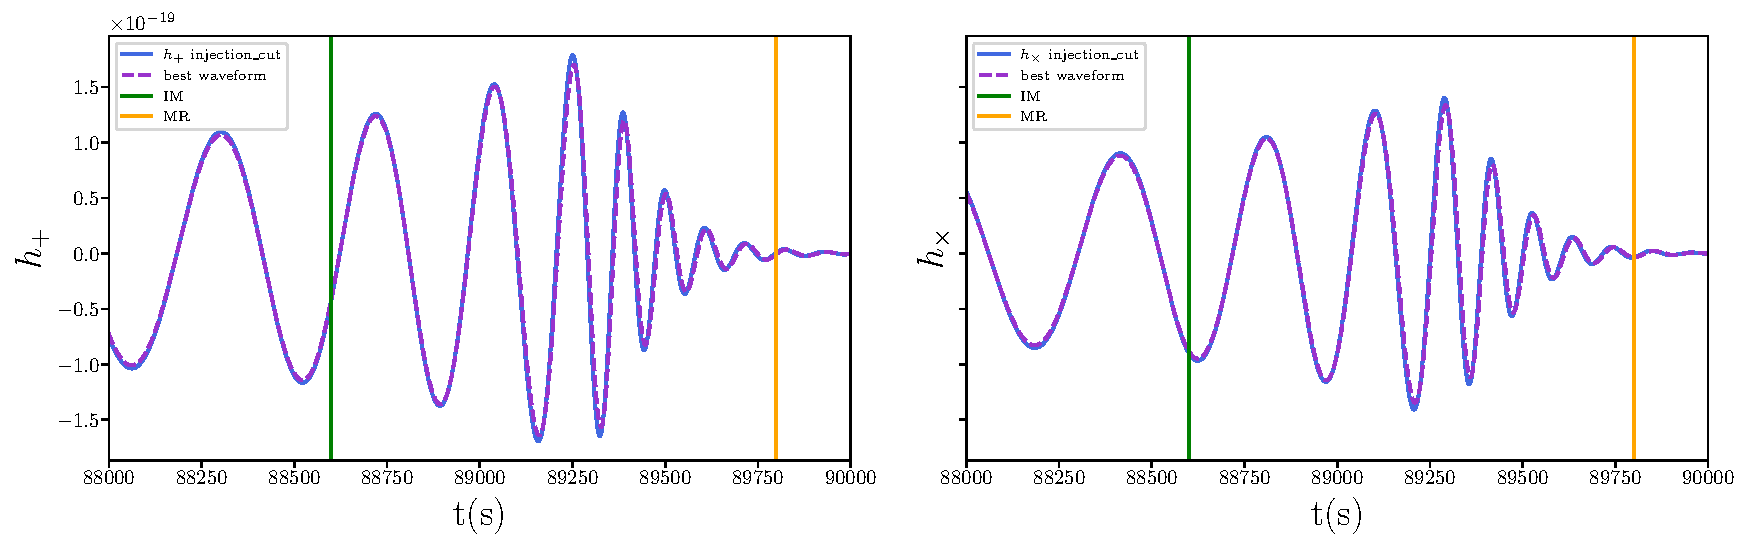
\includegraphics[width=1\textwidth]{Images/Inj_best_insp.pdf}
    \caption{Comparison between the injection signal, blue lines, and the best inspiral parameters waveform, purple dashed lines, presented in form of $h_{+}$ and $h_{\times}$. Vertical lines are the divisor between different parts of the signal, IM = inspiral-merger; MR= merger-ringdown. }
    \label{fig:Inj_best_insp}
\end{figure}



\subsection{Residuals and guess wavelet}

As we have already discussed in sec. \ref{Bayesian_Analysis}, we modify the model used to describe the GW signal by introducing a variable number of wavelets. We decide to fix the parameters that describe the signal without the wavelets, to the maximum $\log \mathcal{L}$ values obtained in the sampling run until $f_{cut}$. From this point onwards, we will only target the fractional deviation and the wavelet parameters.

Before performing the actual parameters samplings, we want to look at the mismatch between the injection signal and the best inspiral waveform, i.e. the residuals and to see if a wavelet, whose parameters are guessed by us in the prior range, can reproduce the residuals. This procedure is done to probe if our idea could possibly work before proceeding with further runs and to help us to choose the prior range for the Bayesian analysis. 

The residuals are shown in Fig. \ref{fig:Residuals}, where the mismatch is the difference between the time domain $h_{+}$, in blue, and $h_{\times}$, in orange. 

\begin{figure}[h!]
    \centering
    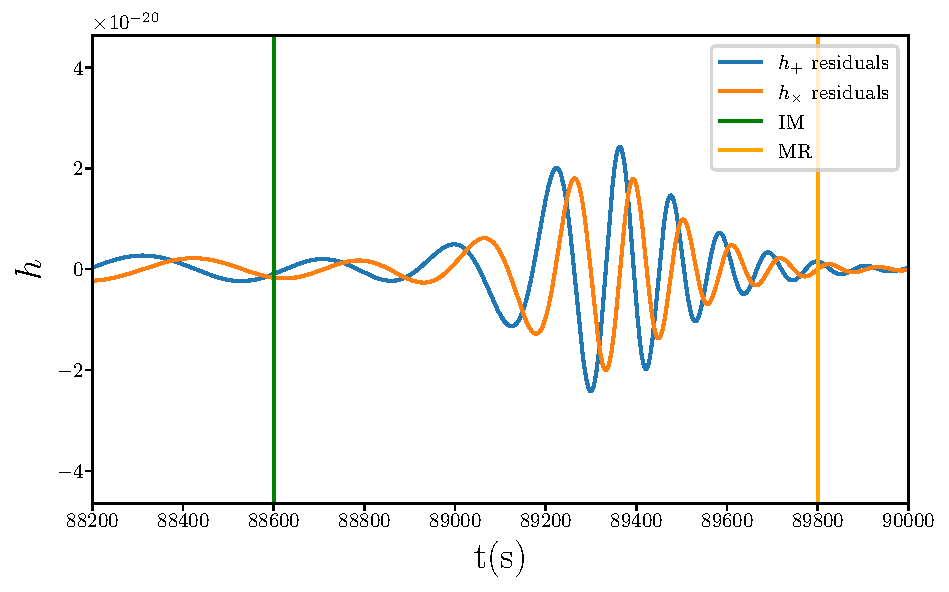
\includegraphics[width=0.7\textwidth]{Images/Residuals.pdf}
    \caption{Residuals, between the injection signal and the best inspiral waveform, shown in time domain. $h_{+}$ is in blue, and  $h_{\times}$ in orange. Vertical lines are the divisor between different parts of the signal, IM = inspiral-merger; MR= merger-ringdown. }
    \label{fig:Residuals}
\end{figure}

We choose flat priors for the five wavelet parameters, between the ranges in table \ref{tab:guess_ranges}: 

\begin{table}[h]
\centering
\begin{tabular}{cc}
\hline
\textbf{Parameter} & \textbf{Range} \\
\hline
$\xi$ & $[ 200\,M; 400\,M]$ \\
$A$ & $[0,\; \max(|h|)] $ \\
$\phi$ & $[-\pi,\; \pi]$  \\
$\nu$ & $[0,\; 10^{-3} \cdot (2\times10^7 / M)]$ \\
$\tau$ & $[1.1\,M,\; 70\,M]$ \\
\hline
\end{tabular}
\caption{Wavelets prior ranges}
\label{tab:guess_ranges}
\end{table}

In Fig. \ref{fig:Guess}, we show the same plot as Fig. \ref{fig:Inj_best_insp} with the addition of the guess wavelet in dashed red, i.e. the wavelet whose parameters were chosen in the prior ranges. The green waveform is described by the full model in eq. \ref{eq:full_model}, with the best inspiral and guess wavelets parameters. We restricted the visualization to a small time region of the merger to have a look at how the waveforms are different. About the $\log \mathcal{L}$ comparison, we started from a value of $ -2377.59 $ and with the guess wavelet we have $\log \mathcal{L} = -1801.84 $. The improvement is not a surprise since we added a new part to the model specifically to address the previous mismatch.

\begin{figure}[h!]
    \centering
    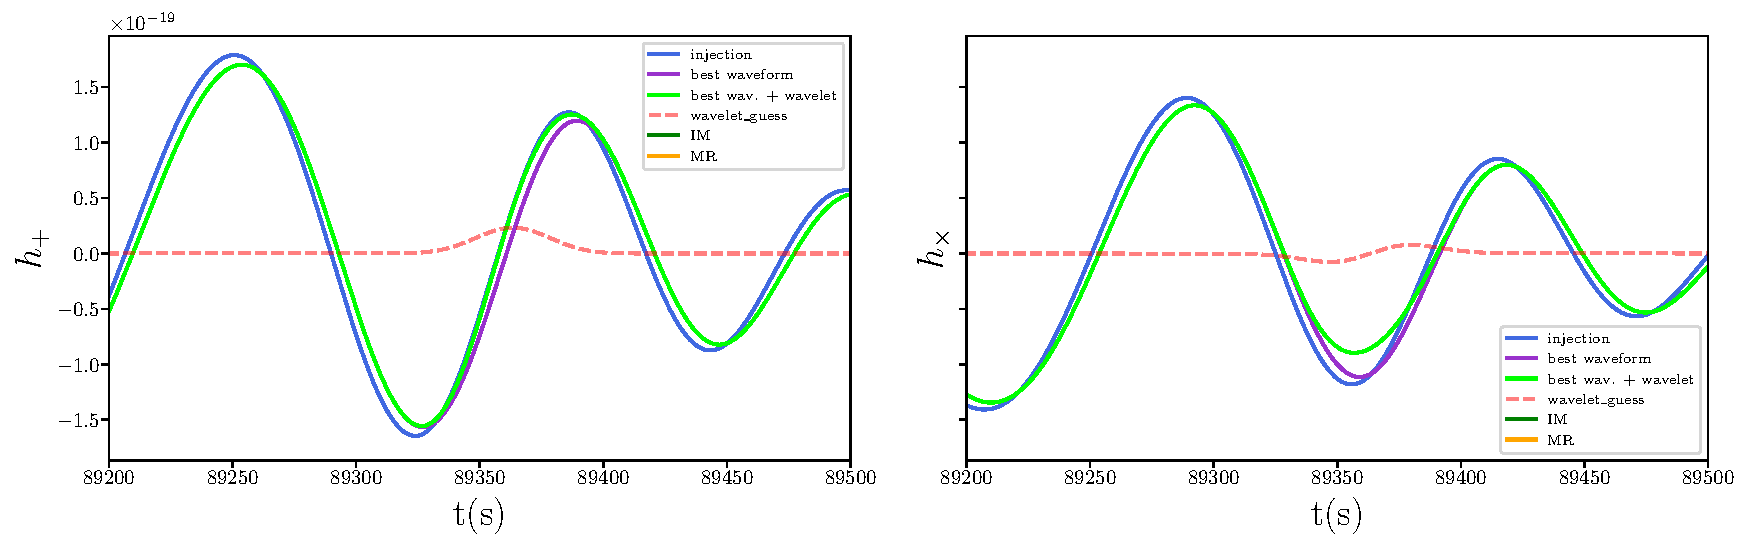
\includegraphics[width=1\textwidth]{Images/Guess.pdf}
    \caption{Comparison between the injection signal, blue lines, and the best inspiral parameters waveform, purple dashed lines, and the best inspiral waveform plus guess wavelet in green; presented in form of $h_{+}$ and $h_{\times}$.  }
    \label{fig:Guess}
\end{figure}




\subsection{Deviations as free parameters}

When defining the best inspiral waveform, we imposed the fractional deviations to be zero. Now, we want to treat these two variables as free parameters for the Bayesian sampling. Firstly, as has already been shown, the injection waveform can be better reconstructed at the cost of biasing these non-GR parameters. Performing a sampling run only for the deviation parameters will allow us to establish a baseline for comparison when wavelets are introduced, quantifying whether the wavelets actually absorb the biases. 

We use the \texttt{Eryn} sampler, with the same number of steps. The initial walkers' positions, both for $\delta f_{22}$ and $\delta \tau_{22}$, are initialized by drawing from a Gaussian distribution $\mathcal{N}(\mu = 0,\, \sigma = 0.005)$. If these values fall outside the prior range, they are drawn from their uniform priors. 

The result of the run can be summarized by the corner plot in Fig. \ref{fig:Corner_dev}. The posteriors show that the deviation parameters are recovered with a bias to match the injection waveform, indicating significant deviations from GR, i.e. the values are not consistent with zero. The $\log \mathcal{L}$ maximum value reached is $-1453.30$, indicating a significant improvement in waveform reconstruction.

\begin{figure}[h!]
    \centering
    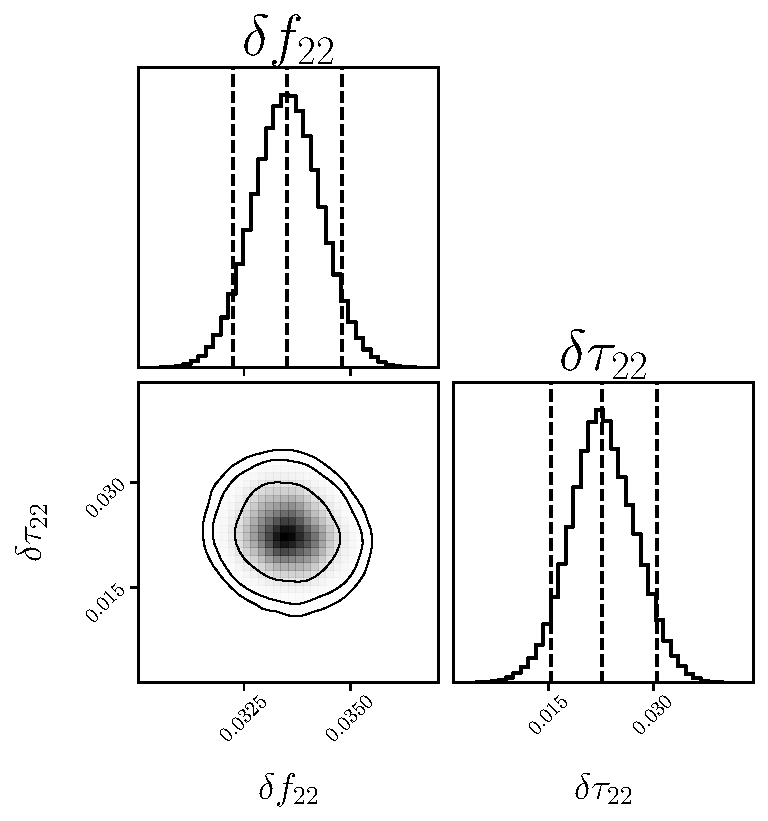
\includegraphics[width=0.7\textwidth]{Images/Corner_dev.pdf}
    \caption{Corner plot of $\delta f_{22}$ and $\delta \tau_{22}$, where all the other parameters are fixed. Contours show the $68\%$, $90\%$, and $95\%$ confidence intervals. The black dashed lines represent the $0.05$, $0.5$, and $0.95$ quantiles.}
    \label{fig:Corner_dev}
\end{figure}




\subsection{Runs with deviations and N wavelets}

In this section, we present the result of several Bayesian parameter estimation runs, with a number of wavelets going from one up to four. In each one of these runs, fractional deviation parameters are also sampled, so the number of sampled parameters is $ 2 + 5 \, N $, where $N$ is the number of wavelets included in the model. Due to the rising of complexity, some of these runs include an higher number and longer burn-in phases, together with more iterations of the sampling run. "These decisions have been made by examining whether the parameter chains have converged.

In addition to extending the sampling runs, we implemented several techniques to improve the convergence of the sampler within a reasonable timeframe. We observed a consistent pattern: runs with different numbers of wavelets tend to converge to the same region in parameter space. Based on this observation, we initialize the walkers' positions for the $N+1$ wavelet run by reusing the high-density region obtained from the $N$-wavelet run, for the first $N$ wavelets. The remaining wavelet is initialized by drawing from the prior distribution. If this strategy is still insufficient to ensure convergence in a run with $N$ wavelets, we restart a second $N$-wavelet run, initializing the walkers with the final state of the previous, non-converged run.



In Fig. \ref{fig:Corner_wav}, we can see the corner plot for the $\delta f_{22}$ and $\delta \tau_{22}$ parameters, being explored during the run. Each color represents a different scenario, where in the model we included a different number of wavelets. The black distributions are the same plotted in Fig. \ref{fig:Corner_dev}, useful for the comparison. As we can see, the addition of just one wavelet shift the posterior distribution of the fractional deviations toward zero, suggesting that the biases in the QNM can actually be absorbed. Going to higher $N$, $\delta f_{22}$ posterior continues to shift toward zero even though we are very far from an effective unbiased frequency, i.e. $\delta f_{22}$ = 0. Instead $\delta \tau_{22}$ distributions start to show biases from two wavelets and so on, shifting from positive biases to negative biases. 

Focusing on $\delta \tau_{22}$, we can observe that the yellow posterior, i.e. four wavelets, has its maximum value nearer to zero with a broader distribution, rather than the two and three wavelets, suggesting that further increase in the number of wavelets could absorb the non-GR biases, at least for the damping time. 



\begin{figure}[h!]
    \centering
    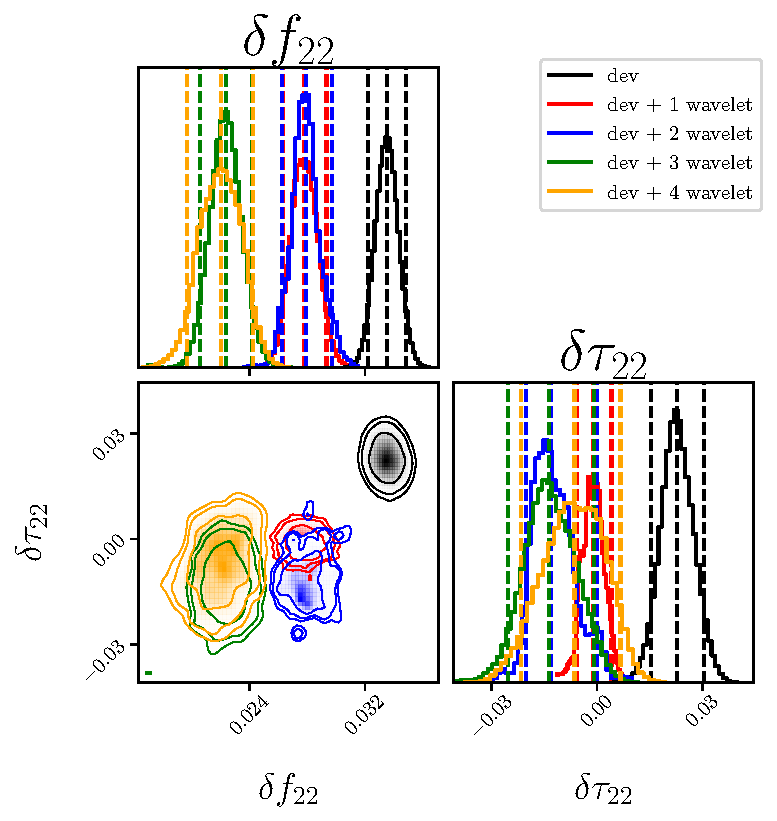
\includegraphics[width=0.7\textwidth]{Images/Corner_wav.pdf}
    \caption{Corner plot of $\delta f_{22}$ and $\delta \tau_{22}$, where all the other parameters are fixed, except for the wavelets. Contours show the $68\%$, $90\%$, and $95\%$ confidence intervals. The dashed lines represent the $0.05$, $0.5$, and $0.95$ quantiles. Each color refers to a run with $N$ wavelets and deviations: red for 1, blue for two, green for three, and  yellow for four wavelets.}
    \label{fig:Corner_wav}
\end{figure}


We give a summary statistic of the four wavelets scenario: 

\begin{equation}
\delta f_{22} = 0.022^{+0.002}_{-0.002} \,, \quad 
\delta \tau_{22} = -0.006^{+0.013}_{-0.015} \,;
\end{equation}

\noindent 

where we report the $0.05$, $0.5$, and $0.95$ quantiles of the posterior distribution, defining a $90\%$ credible interval. At least, the $90\%$ credible interval for $\delta \tau_{22}$ includes the GR scenario.

Looking at Fig. \ref{fig:Inj_4wav}, we have a visual comparison between the injection signal, the best inspiral waveform, and the waveform created when we include the maximum $\log \mathcal{L}$ QNM deviations and wavelet parameters. This comparison is presented in form of $h_{+}$ and $h_{\times}$. There are also plotted the single wavelets as dotted-dashed lines.


\begin{figure}[h!]
    \centering
    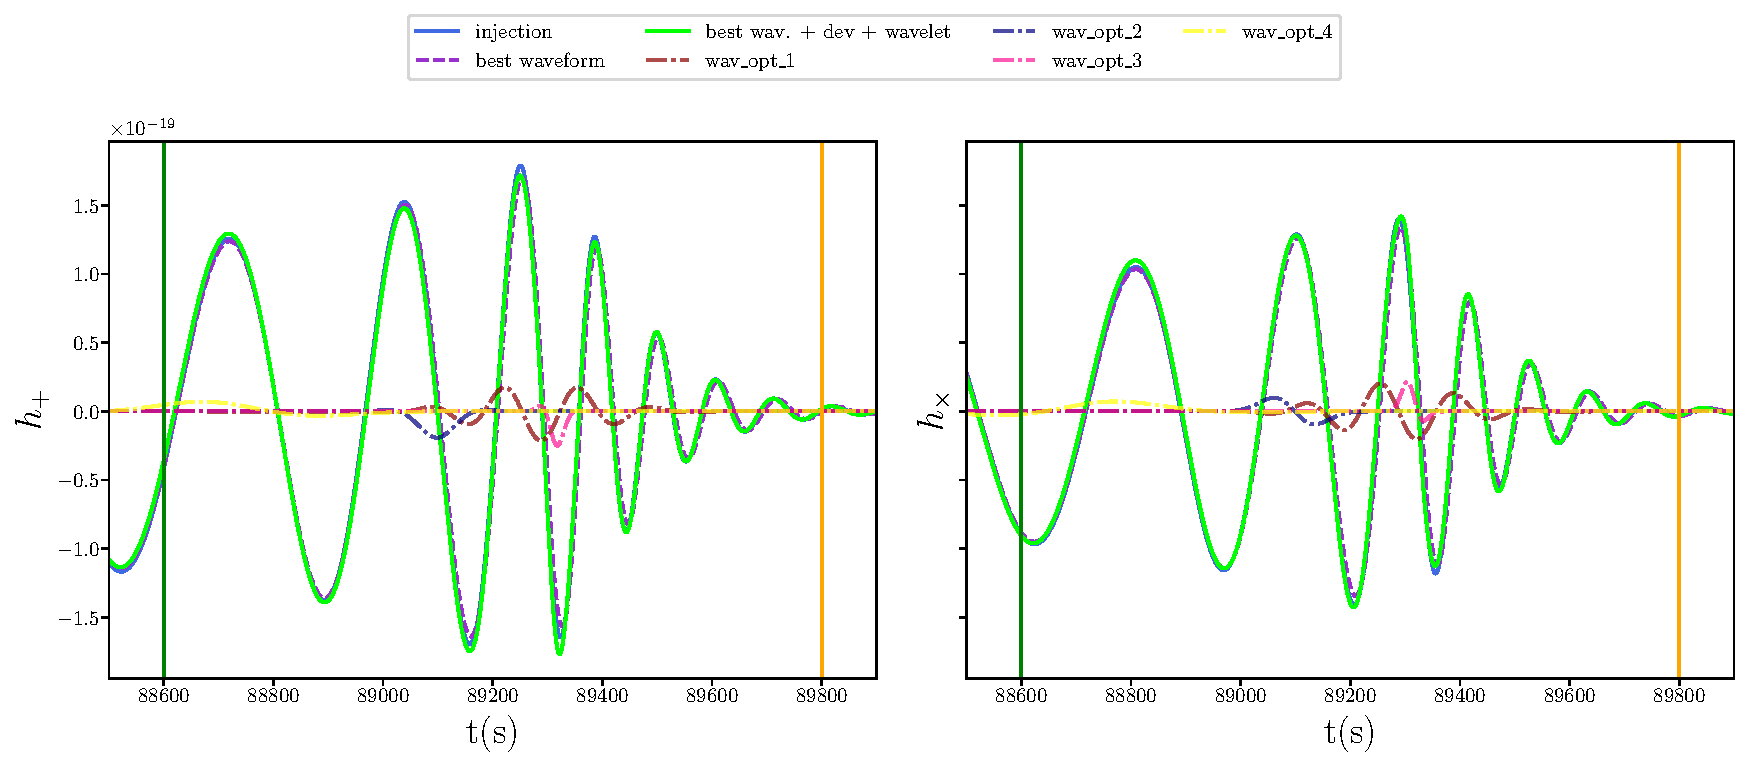
\includegraphics[width=1\textwidth]{Images/Inj_4wav.pdf}
    \caption{Comparison between the injection signal, blue lines, and the best inspiral waveform, purple dashed lines, and the 4 wavelets + deviations waveform, green line, presented in form of $h_{+}$ and $h_{\times}$. Vertical lines are the divisor between different parts of the signal, IM = inspiral-merger; MR= merger-ringdown. The dotted-dashed lines are the four wavelets added to the model.}
    \label{fig:Inj_4wav}
\end{figure}
 
 
\subsection{Model selection}
In the previous section we focused on modifying our recovery model, by increasing the number of wavelets, in order to absorb the biases presented in QNM fractional deviations, since we know that the injection signal is fully described by GR. Doing that we postpone the discussion about which model should be favoured, since models with a higher number of wavelets best adapts to the injection but they are more complex, since each new wavelet is characterized by five parameters.

In order to answer this question, we can resort to the Akaike Information Criterion (AIC) \cite{1100705}. The AIC is defined as follows:

\begin{equation}
\mathrm{AIC} = 2\,n_{\mathrm{fp}} - 2\,\max\left( \log \mathcal{L} \right)
\end{equation}

\noindent
where $n_{\mathrm{fp}} = 2 + 5 \, N $ is the number of free parameters, that accounts for the dimensionality penalty, trying to avoid overfitting models. When choosing between different models to describe observed data, the one with minimum AIC is favoured. We computed the AIC for all the models described before, we show the results in Fig. \ref{fig:AIC}. From these results, even acknowledging these models did not manage to absorb false GR deviations, we should prefer the most complex model, i.e. deviations and four wavelets, among the others. The AIC trend suggests that adding more wavelets to the model may be favoured, until the increase in complexity is no longer justified by the increase in the $\log \mathcal{L}$, though always considering the rise in computational cost and feasibility.


\begin{figure}[H]
    \centering
    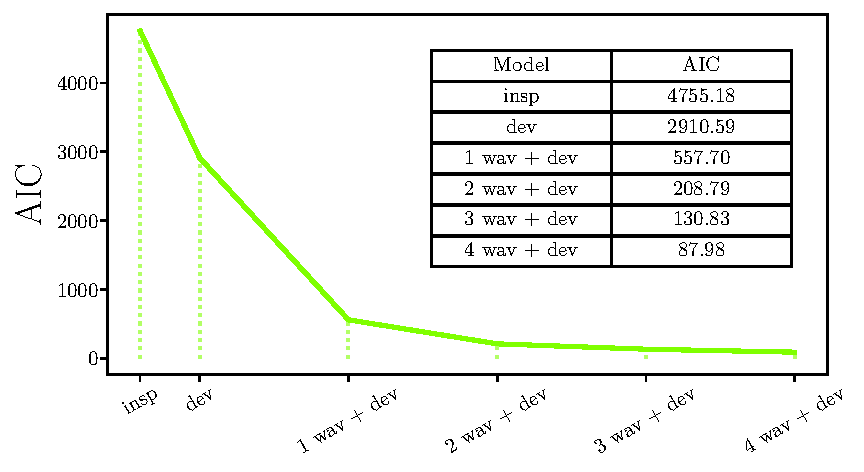
\includegraphics[width=0.7\textwidth]{Images/AIC.pdf}
    \caption{AIC computation for different scenarios: only best inspiral, only deviations, and deviations plus $N$ wavelets.}
    \label{fig:AIC}
\end{figure}
